\section{Methodology} \label{sec:methods}

The images used contain standard \textit{overscan}, \textit{bias}, \textit{dark}, and \textit{defects} reduction, which consist of maps indicating regions with both bright and dark defects, eg. dead pixels. The above reduction corresponds to the starting state for the PTC study. Subsequently, other corrections such as \textit{linearity} and \textit{crosstalk} are made to analyze their effects on the main parameters of the camera.

\vspace{3mm}

Professor Craig Lage generated supercalibrations for the entire focal plane, which are in a chain in his personal collection \textit{u/cslage/calib/13144/calib.20220103}. Whereas, the images shown in Figures \ref{fig:superbias} and \ref{fig:superdark} are superbias and superdarks (left panel E2V and right panel ITL), respectively, which were generated as part of the learning process for producing the calibration images using the software developed for the LSST, called \textit{DM stack}.

\vspace{3mm}

The code with which the calibration images are generated via \textit{DM stack} can be found in \\  \href{https://github.com/lsst/cp_pipe}{https://github.com/lsst/cp\_pipe}, and it generates the data for the construction of the PTC, calculates the gain for each CCD segment as its FWC. In addition, it calculates the gain by another different method, which was analyzed in section \ref{subsec: method_gainflat} to determine the differences between it and the PTC, which consists of using two pairs of flats for its estimation. We use two code versions of the \textit{DM stack}\footnote{DM stack is the software developed for the LSST and is publicly available on GitHub, and it can be found at \href{https://github.com/lsst/}{https://github.com/lsst/}},  for the entire focal plane: 


\begin{itemize}
    \item w\_2022\_27: Initial version we started working with. 
    \item w\_20222\_32: Version that couples one of our main results on obtaining the gain with pairs of flats (see the \href{https://jira.lsstcorp.org/browse/DM-35790}{DM-35790} ticket in Jira ).
\end{itemize}

BPS (Batch Processing Service) was used to run the two previous versions. The details of how to build the configuration files, possible errors, associated link for more information, and how to use the obtained data can be found in the GitHub repository of this project \href{https://github.com/linagiraldom/RECA_Internship_Project}{RECA\_Internship\_Project} in the notebook \href{https://github.com/linagiraldom/RECA_Internship_Project/blob/main/Notebooks/BPS_LSST.ipynb}{BPS\_LSST.ipynb}. In addition, all notebooks used to carry out the methodology described below are available in this repository. There is also a notebook called \href{https://github.com/linagiraldom/RECA_Internship_Project/blob/main/Notebooks/Tutorial.ipynb}{Tutorial.ipynb} where I explain a little bit about the \textit{Data Butler}, which is the API that manages and stores the data, where to find more information about it, what are the collections, visualize images, get the data and work with them, among other details about the calibration images.



\begin{figure}[!htb]
     \centering
     \begin{subfigure}[b]{0.49\textwidth}
         \centering
         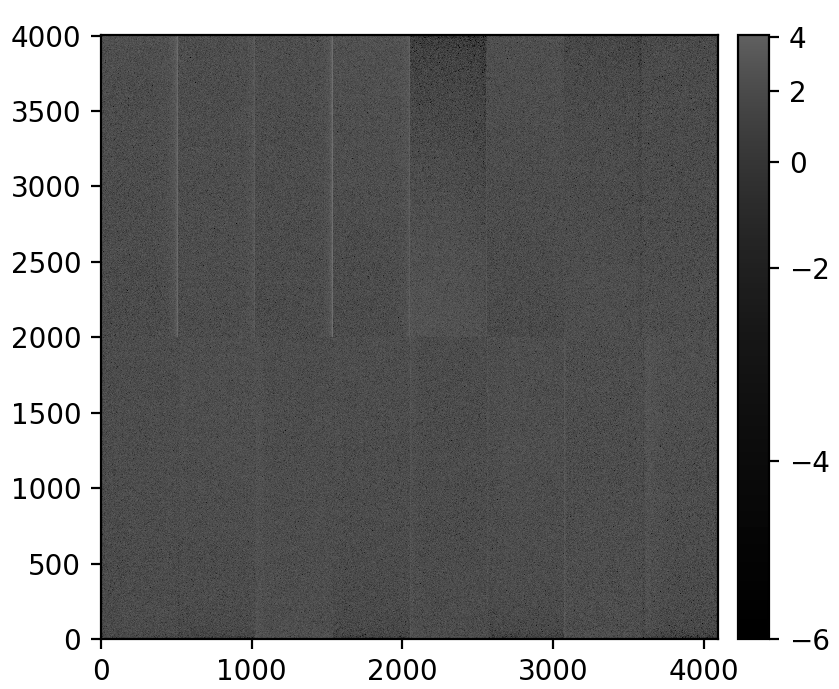
\includegraphics[width=\textwidth]{Figures/Super_bias_55.png}
     \end{subfigure}
     \hfill
     \begin{subfigure}[b]{0.49\textwidth}
         \centering
         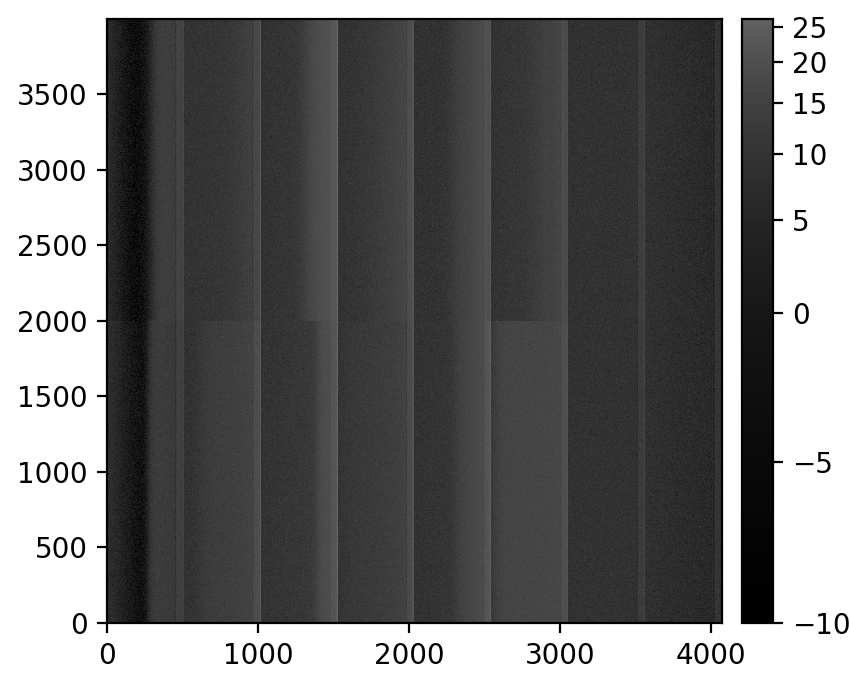
\includegraphics[width=\textwidth]{Figures/Super_bias_74.png}
     \end{subfigure}
        \caption{Masterbias for detectors 55 (E2V), on the left and 74 (ITL), on the right. }
        \label{fig:superbias}
\end{figure}

\begin{figure}[!htb]
     \centering
     \begin{subfigure}[b]{0.49\textwidth}
         \centering
         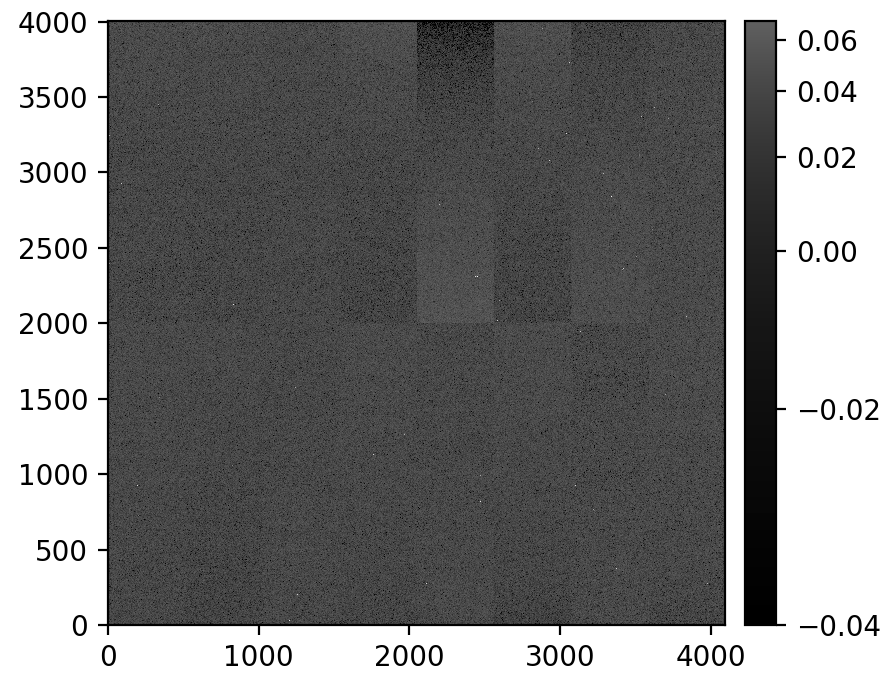
\includegraphics[width=\textwidth]{Figures/Super_dark_55.png}
     \end{subfigure}
     \hfill
     \begin{subfigure}[b]{0.49\textwidth}
         \centering
         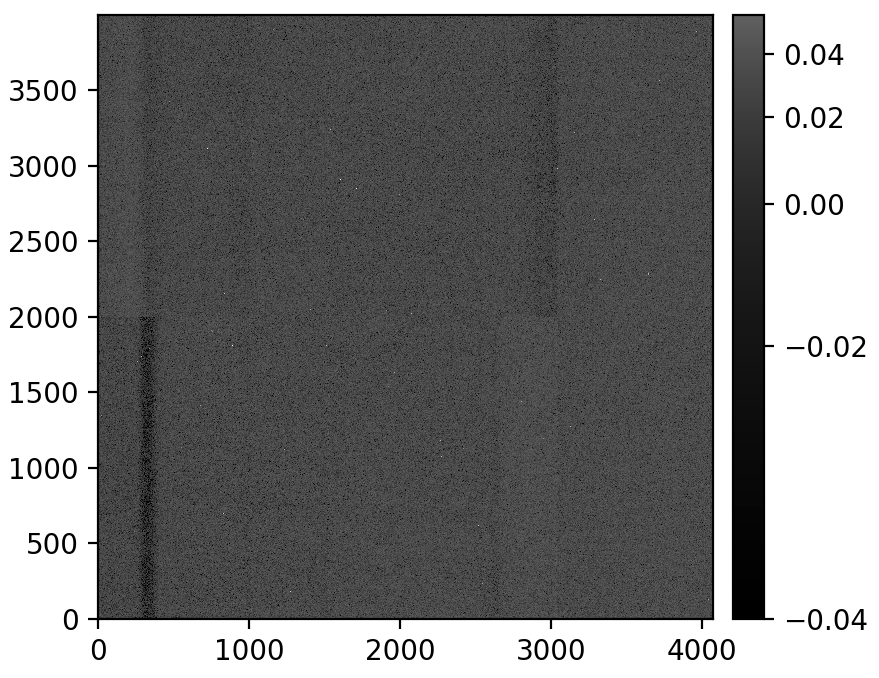
\includegraphics[width=\textwidth]{Figures/Super_dark_74.png}
     \end{subfigure}
        \caption{Masterdarks for detectors 55 (E2V), on the left and 74 (ITL), on the right.}
        \label{fig:superdark}
\end{figure}


\subsection{Photon Transfer Curve (PTC)}

The PTCs were generated for the whole LSSTCam focal plane using  \textit{DM stack}\footnote{The PTCs are constructed with the code available in the repository \href{https://github.com/lsst/cp_pipe}{cp\_pipe}}, which allows estimating the gain, the read noise, $a_{00}$ (parameter related to the B-F effect) and the turnoff (associated with the Full Well Capacity, FWC) from a fit to the shape of the PTC. This code implements equations 16 and 20 of the \cite{astier2019shape} article: equation 16 corresponds to the exponential approximation (EXPAPPROXIMATION), which uses only the variance ($C_00$); while equation 20 is the full model (FULLCOVARIANCE), and implements the covariance matrix. In this work, we used EXPAPPROXIMATION, whose equation is as follows

\begin{equation}
    C_{00} = \frac{1}{2 g^2 a_{00}} [\exp (2 a_{00} \mu g) - 1] + \frac{n_{00}}{g^2}
    \label{eq:Astier16}
\end{equation}

where $C_{00}$ is the variance, $g$ is the gain, $a_{00}$ is always negative and is related to the B-F effect, $mu$ is the mean, and $n_{00}$ ($el^{2}$) is the noise. According to \cite{astier2019shape}, $a_{00}$ being negative leads to the variance of a flat field not growing as fast as the mean does. In the case where there is no B-F effect, i.e., each pixel is independent of the other and is described by a Poisson statistic, the mean, gain, and variance are directly related through 

\begin{equation}
    V = \frac{\mu}{g}
    \label{eq:gain_Poisson}
\end{equation}

where $V$ is the variance of a flat field, $mu$ is the mean, and $g$ is the gain.

\subsection{Gain from flat pairs} \label{subsec: method_gainflat}

An independent method for calculating a sensor's gain is using flat field pairs with equal exposure times. Since each CCD is composed of 16 segments, each with its amplifier, a gain value is obtained for each segment. For this purpose, the LSST has the function \href{https://github.com/lsst/cp_pipe/blob/main/python/lsst/cp/pipe/ptc/cpExtractPtcTask.py#L679}{Gain from flat pairs}, which was analyzed in detail in this work. 

\vspace{3mm}

We aim to quantify the difference between the gain calculated from the fit to the PTC and this method. For this, we initially calculate the average flux in ADU with each flat pair, the read noise, and the gain. The latter is estimated employing the equation of \cite{lupton2014consequences}

\begin{equation}
    \frac{1}{g} = \Big \langle \frac{(I_1 - I_2)^2}{I_1 + I_2} \Big \rangle 
    \label{eq:Lupton}
\end{equation}

Where $g$ is the gain, $I_1$ is the first flat image, and $I_2$ is the second flat image, both at the same exposure time. The expected value over all pixels is the inverse of gain. Considering the corrections for read-out noise, the equation takes the following quadratic form:

\begin{equation}
    \frac{1}{g} = \Big \langle \frac{(I_1 - I_2)^2}{I_1 + I_2} \Big \rangle - \frac{1}{\mu} (N^2-\frac{1}{2} g^2)
    \label{eq:gain_corrected}
\end{equation}

where $mu = 0.5(\mu_1 + \mu_2)$ with $mu_1$ and $mu_2$ the average value for each of the flat images and $N$ is the read-out noise. This above equation has three variants: NONE, SIMPLE and FULL, with NONE being equal to the equation \ref{eq:Lupton}. The remaining two cases are as follows:

\begin{align}
g = \begin{cases}
  \frac{1}{K - \frac{1}{\mu}(N^2 - \frac{1}{2} g^2)} & \mbox{SIMPLE} \\
  \frac{\mu + \sqrt{\mu^2 - 2 \mu K + 2 N^2}}{2 K \mu - 2 K^2} & \mbox{FULL}
\end{cases}
\label{eq:sol_gain_corrected}
\end{align}

where $K$ is equal to the equation \ref{eq:Lupton}. In the SIMPLE case $g = 1/K$, while in the FULL case the quadratic equation is solved and the result is taken to have physical meaning. Once we have the gains calculated from pairs of flats for flows between 0 and $\sim 10000$ ADU, we calculated the relative percentage error with the gain obtained with the fit to the PTC. We use the equation \ref{eq:sol_gain_corrected} with FULL type correction to calculate this relative error, thus:

\begin{equation}
    \mbox{Relative\_error} [\%] = \frac{|gain_{PTC} - gain_{flats}|}{gain_{PTC}} \times 100 \% 
    \label{eq:error_relativo_gain}
\end{equation}


Subsequently, a linear low-flow fit was performed, which we considered being between 5000 and 10000 ADU. The low-flow fit has the following form: 

\begin{equation}
    \mbox{Relative\_error}_{LF} [\%] = m F + \mbox{offset}
\end{equation}

where $m$ is the slope of the fit, $F$ is the flux, and  \textit{offset} is the intercept with the $y$-axis. These parameters serve us to quantify the error variation in this flow range and the base error between the PTC gain and that calculated with the flats. We made histograms of these parameters to see the vendor's behavior and extract a general behavior. This is calculated by leaving out the outliers, i.e., the CCD segments with abnormal behavior. To do this, we made use of \cite{price2018astropy} and its functions \textit{sigma\_clip} and \textit{sigma\_clipped\_stats} with which we cut the data so that those that were within $3 \sigma$ of the median were kept and we iterated three times. 



 \begin{figure}[!htb]
     \centering
     \begin{subfigure}[b]{\textwidth}
         \centering
         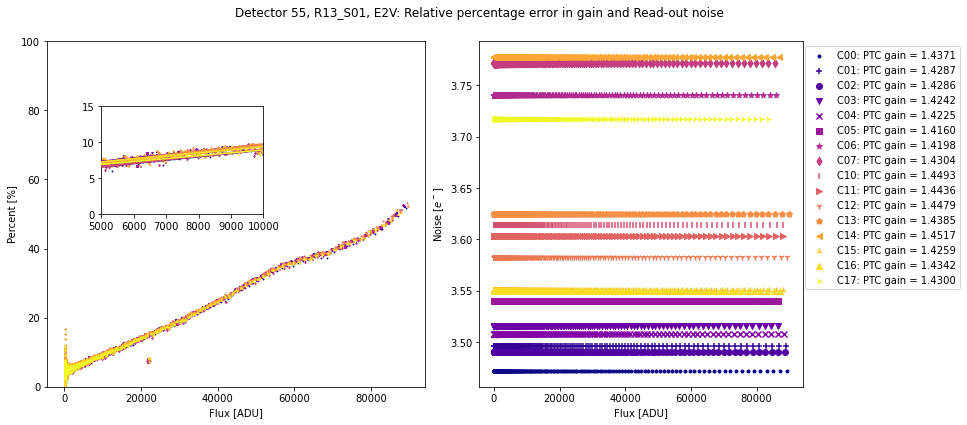
\includegraphics[width=\textwidth]{Figures/Relative_Error_Gain_Noise_detectorR13_S01_old.png}
     \end{subfigure}
     \vspace{3mm}
     \begin{subfigure}[b]{\textwidth}
         \centering
         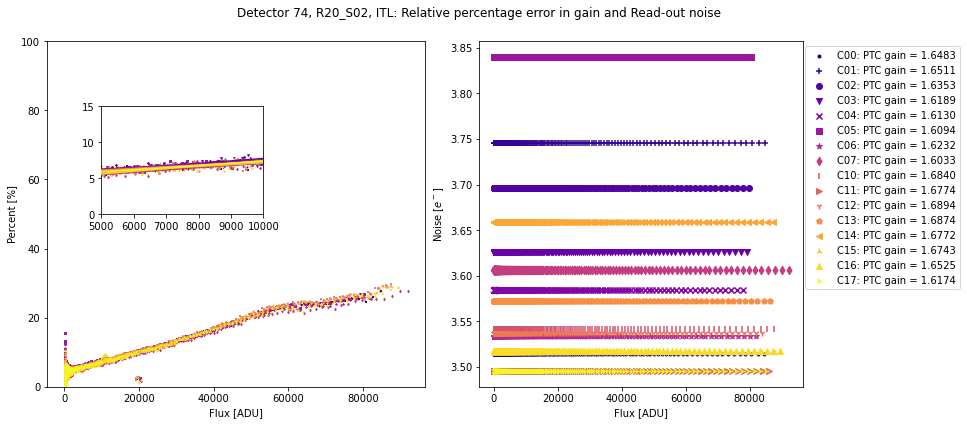
\includegraphics[width=\textwidth]{Figures/Relative_Error_Gain_Noise_detectorR20_S02_old.png}
     \end{subfigure}
        \caption{Relative percentage error between the gain estimated by the PTC and the gain calculated from two flat images (left), and the read-out noise of each amplifier (right), using the initial code. In the upper panel, it is shown for detector 55 (R13\_S01), whose vendor is E2V, and in the lower panel for detector 74 (R20\_S02) from the vendor ITL. Each color and symbol represents the relative percentage error for one of the 16 segments that make up each CCD. The embedded image in the left panels shows the percentage error between 5000 and 10000 ADU (low flux regime), in which a linear fit is made. The data used to construct these plots consider only those below the PTC turnoff.}
        \label{fig:relative_error_oldcode}
\end{figure}


\begin{figure}[!htb]
    \centering
    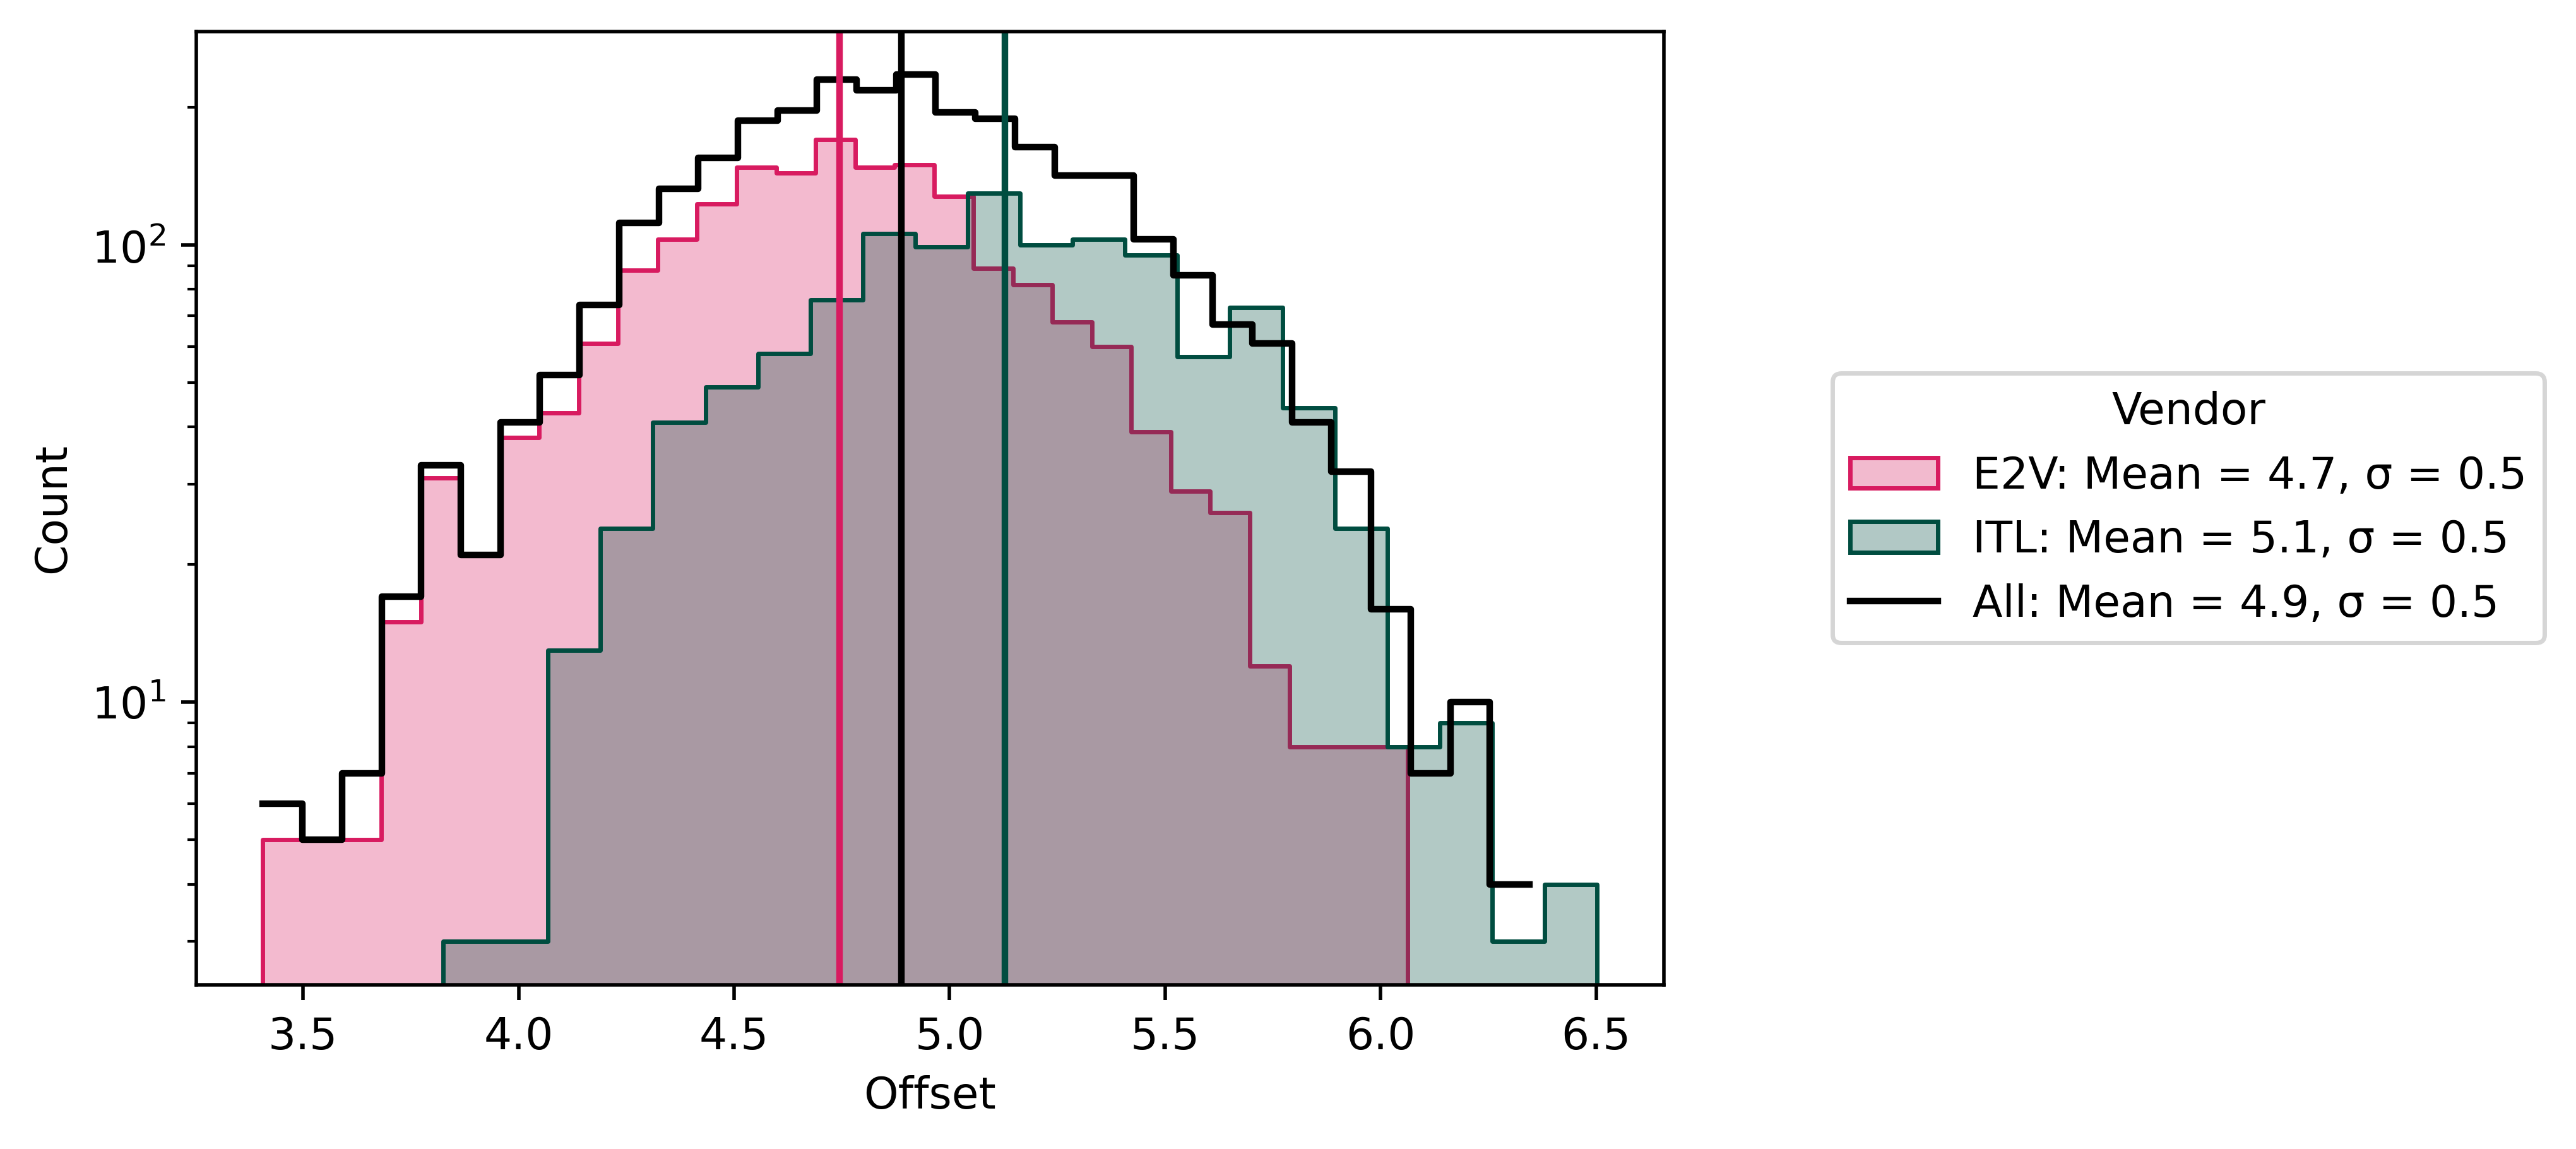
\includegraphics[width=\textwidth]{Figures/Histogram_offset_old.png}
    \caption{Histograms with the offset value obtained from the linear fit for flows between 5000 and 10000 ADU for the relative percentage error between gains. In magenta is shown the distribution for E2V, with a mean of $(4.7 \pm 0.5)$ \%, and in blue for ITL, with a mean of $(5.1 \pm 0.5)$ \%. The distribution in black represents the histogram of all data without discriminating by vendor, with a mean of $(4.9 \pm 0.5)$ \%. The vertical lines represent the value of the mean for each of the distributions.}
    \label{fig:hist_offset_old}
\end{figure}

\subsubsection{Simulation} \label{subsubsec:method_Simulation_Gain}

The methodology described in section \ref{subsec: method_gainflat} and the use of the LSST software version \textit{w\_2022\_27} led us to the results seen in Figures \ref{fig:relative_error_oldcode} and \ref{fig:hist_offset_old}. Figure \ref{fig:relative_error_oldcode} shows the relative percent error between the gains over the flow range below the PTC turnoff for E2V sensor 55 (top panel) and ITL sensor 74 (bottom panel). The figure for each sensor has on the left an embedded plot showing the behavior between 5000 and 10000 ADU with its respective linear fit; on the right is the error of each of the CCD segments for the same flow range.  We see in the embedded plot that the relative error has an offset higher than 5 \% for these two sensors, so we made a histogram with the offset values for the entire focal plane and verified if this behavior is generalized. Figure \ref{fig:hist_offset_old} confirms that this relative error, on average, is a behavior exhibited by all sensors. We consider a base error of $\sim 5$ \% to be relatively high, so we decided to investigate this problem through simulations.

\vspace{3mm}

Different variables could cause the problem described above to arise: an over-estimation of the read-out noise, the mask used in the images is affecting, or another factor, such as the assumption that the distribution is Gaussian for the operation between the flat images given by  

\begin{equation}
      \frac{(I_1 - I_2)^2}{I_1 + I_2} 
      \label{eq:ratioIm}
\end{equation}

as it is being assumed in the \textit{w\_2022\_27} version of the \textit{DM stack}. If the distribution is not Gaussian, the distribution statistics are modified. We explored 3 cases through simulation to rule out or confirm variables, as described below:

\begin{itemize}
    \item \textbf{Case 1 - Noise over-estimation}: Two data sets were constructed following a Poisson distribution for the flow, with an expected value between 5000 and 10000 ADU. In our case, we chose 5000 ADU. The distribution is then:
    
    
    \begin{equation}
        f(k;\lambda) = \frac{\lambda^k e^{-\lambda}}{k!} \implies f(k;5000) = \frac{5000^k e^{-5000}}{k!}
    \end{equation}
    \label{eq:dist_Poisson}
    
    
where the expected value is $\lambda$, and $k$ is the number of events. To the data following this distribution, we add a Gaussian noise whose mean is zero, and the value which gives the dispersion we will assume as the read-out noise, that is:

\begin{equation}
    p(x) = \frac{1}{\sqrt{2 \pi \sigma^2}} \exp \Big(-\frac{(x - \mu)^2}{2\sigma^2} \Big) \implies p(x) = \frac{1}{\sqrt{2 \pi N^2}} \exp \Big(-\frac{x^2}{2N^2} \Big)
    \label{eq:gaussian_noise}
\end{equation}

where the mean is $mu$, $sigma$ is the standard deviation, and $N$ is the read-out noise, which we assume. Finally, we employ the methodology described in \ref{subsec: method_gainflat} for all types of gain correction: NONE, SIMPLE and FULL, and calculate the relative error using a base gain (we choose a value of 2.0) to verify if we can recreate what is observed in figure \ref{fig:relative_error_oldcode}, i.e., a base error above 5 \%.

\item \textbf{Case 2 - Pixel masks}: As a next step, pixel masks are added to case 1. For this, the respective mask is extracted from each flat image, where each flat has an average of $5000$ ADU counts. This mask filters out suspicious, bad, dead, and saturated pixels. A Poisson distribution is then generated with the dimensions of one of the CCD segments for which the masks were extracted, that is, $size_x = 2002$ and $size_y = 512$, with its respective Gaussian noise. The respective mask is applied to each array using the \textit{Numpy} function \citep{harris2020array} \textit{ma.masked\_where}.


\begin{figure}[!htb]
    \centering
    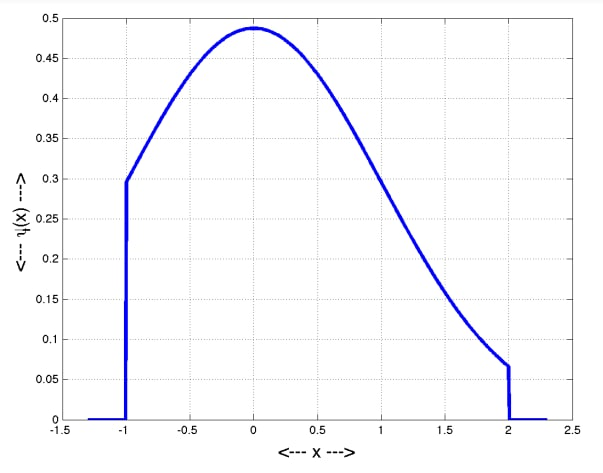
\includegraphics[width=0.5\textwidth]{Figures/Truncated_Gaussian.jpg}
    \caption{Truncated Gaussian distribution with both zero mean and standard deviation, $\psi(0,1,a = -1, b = +2; x)$. Figure is taken from \cite{burkardt2014truncated}.}
    \label{fig:truncated_gaussian_dist}
\end{figure}


\item \textbf{Case 3 - Statistics control}: To case 2, we add statistics control, i.e., we assume that the distribution of \ref{eq:ratioIm} is Gaussian, and we cut the distribution as it was done in the section \ref{subsec: method_gainflat}, only in this case we keep all the data that are within $5.5 \sigma$ of the mean, and we perform three iterations. Suppose the distribution of \ref{eq:ratioIm} is Gaussian. In that case, it must be satisfied that the mean of the truncated and original distribution is the same if symmetric cuts are made. When truncating non-symmetrically, the mean of this distribution is:

\begin{equation}
    \mu = \overline{\mu} - \overline{\sigma} \frac{\phi (0,1; \beta) - \phi (0,1; \alpha)}{\Phi (0,1; \beta) - \Phi (0,1; \alpha)} \; \; \; ; \alpha = \frac{a-\overline{\mu}}{\overline{\sigma}} , \beta = \frac{b -\overline{\mu}}{\overline{\sigma}}
    \label{eq:truncated_dist}
\end{equation}

where $\alpha$ and $\beta$ are standardized variables, $a$ and $b$ are the cutoff values for each side of the distribution, $\overline{\mu}$ and $\overline{\sigma}$ are the statistics of the original distribution, $\phi$ is the normal PDF, and $\Phi$ is the normal CDF. This case is illustrated in Figure \ref{fig:truncated_gaussian_dist} for $a=-1$ and $b=+2$. However, if $-a=b$, i.e., the distribution is symmetrically truncated, the numerator of the second term in the above equation becomes zero and is reduced to

\begin{equation}
    \mu = \overline{\mu}
    \label{eq:truncated_dist_simetric}
\end{equation}

which implies that the mean of the truncated and the original distribution are equal. Therefore, we use this result to calculate the expected value of the equation \ref{eq:Lupton} and thus find the gain solutions for the NONE, SIMPLE and FULL corrections. As an additional step, we check the shape of the distribution of \ref{eq:ratioIm}; in case it is not Gaussian, no truncation is made to the distribution, and the expected value of the equation \ref{eq:Lupton} is calculated with arithmetic mean. 

\end{itemize}


\subsection{No linearity Correction} \label{subsec:method_Linearity}

To see the effect of linearity correction on the shape of the PTC and its parameters, we used a Spline linearizer with 12 nodes for detectors 32 (ITL) and 139 (E2V). This linearizer was generated by Jeronimo\footnote{Jerónimo was my partner during this internship, who worked on the sister project \href{https://github.com/jerocalderong/LinearityRubinObservatoryCCDs/blob/main/Linearity_of_the_Vera_Rubin_Observatory_CCDs_Prelim.pdf}{Study of the Linearity of the CCDs of the Vera C. Rubin Observatory}} and in his analysis found that a Spline with 12 equally spaced nodes greatly corrects the effect of the nonlinearity and decreases the dispersion in the residuals. All configurations were the same, except, of course, the linearity correction (see table \ref{tab:config_linearity}).


\begin{table}[!htb]
\centering
\caption{Configuration used to generate the PTCs. The linearity correction is performed in this case, ``doLinearize: true''.}
\label{tab:config_linearity}
\resizebox{\textwidth}{!}{%
\begin{tabular}{cccc}
\hline
\multicolumn{4}{c}{\textbf{Configuración}} \\
\hline
\hline
  doWrite: true       &  doLinearize: true      &  doFlat: false       &  doInterpolate: false  \\
  doOverscan: true    &  doCrosstalk: false      &  doFringe: false     &  doSaturation: false   \\
  doAssembleCcd: true &  doBrighterFatter: false &  doApplyGains: false &  doSaturationInterpolation: false  \\
  doBias: true        &  doDark: true            &  doDefect: true      &  growSaturationFootprintSize: 0 \\
  doVariance: true    &  doStrayLight: false     &  doNanMasking: true  &  ptcFitType: EXPAPPROXIMATION \\
  \hline
\end{tabular}%
}
\end{table}

Subsequently, plots of $\frac{Variance}{Mean}$ vs $Mean$ are constructed, so that the variance is normalized. Thus, it is analyzed whether the bump between 50000 and 60000 ADU is corrected. In addition, a relative percentage error between the parameters obtained from the PTC fit with and without correction for linearity is calculated to quantify the effect on these. Finally, we checked whether the parameters and/or the shape of the PTC changed concerning its version without correction for nonlinearity.


\subsection{Crosstalk Correction} \label{subsec:method_Crosstalk}

The full focal plane readout of the LSSTCam can reach a readout time of 2s, so the combination of high speed, high resistivity silicon components, and close spacing between each channel makes the LSSTCam more susceptible than any other mosaic camera to electronic crosstalk \citep{o2015crosstalk}.

\vspace{3mm}

\begin{figure}[!htb]
    \centering
    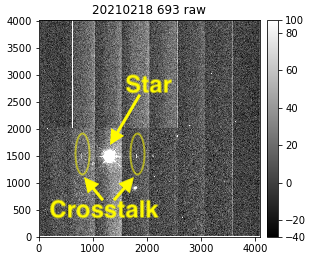
\includegraphics{Figures/Crosstalk_effect.png}
    \caption{Image of a bright star taken with the 1.2m auxiliary telescope at the Vera Rubin Observatory.  Segments adjacent to the bright start image show crosstalk.}
    \label{fig:crosstalk}
\end{figure}

Electronic crosstalk occurs in CCDs that contain several channels that are read simultaneously and coupled so that a channel that detects a bright source will cause a ghost image to be generated in adjacent segments due to this coupling \citep{snyder2020laboratory}. This effect is presented in figure \ref{fig:crosstalk}, where ``ghost'' signals are observed in the lateral segments of the detector. Figure \ref{fig:crosstalk_matrix} shows a heat map on the left for ITL detector 32 and on the right for ITL detector 139, where the highest crosstalk coefficients are in blue colors, and it is observed that the crosstalk pattern is different per vendor. These same coefficients are entered into a configuration file in the LSST software to re-generate the PTC with this correction.

Finally, as in the section \ref{subsec:method_Linearity}, we checked whether the parameters and/or the shape of the PTC changed concerning its version without correction for crosstalk.


\begin{figure}[!htb]
     \centering
     \begin{subfigure}[b]{0.49\textwidth}
         \centering
         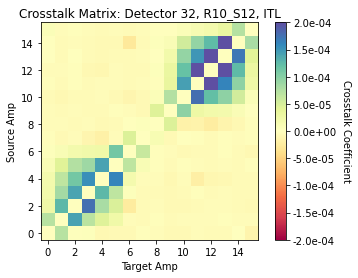
\includegraphics[width=\textwidth]{Figures/Crosstalk_32.png}
     \end{subfigure}
     \hfill
     \begin{subfigure}[b]{0.49\textwidth}
         \centering
         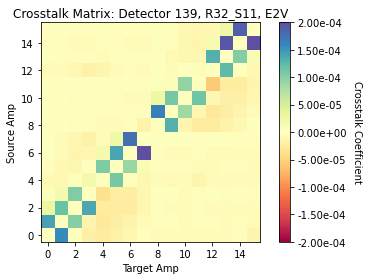
\includegraphics[width=\textwidth]{Figures/Crosstalk_139.png}
     \end{subfigure}
        \caption{Crosstalk matrix on the left for detector 32 (ITL) and on the right for 139 (E2V).}
        \label{fig:crosstalk_matrix}
\end{figure}